\documentclass{article}
\usepackage{graphicx} % Required for inserting images
\usepackage{amsmath, amssymb, amsfonts}
\usepackage{float}
\usepackage{enumerate}
\usepackage{tikz}
\usetikzlibrary{positioning}

\title{latex tutorial2}
\author{Jing Jin }
\date{April 2025}

\begin{document}

\maketitle

\section{math}
Hello world! This is my first latex introduction course! $y =x +1$. Let's explore this
fantastic world together.
$$y =x +1$$
power:
$$x^2$$
subscript:
$$x_{2344}5$$
fraction:
$$\frac{1}{1+\frac{1}{x}}$$
$$\dfrac{1}{1+\dfrac{1}{x}}$$
functions:
$$\log 2$$
$$\log_3 2$$
$$\ln 3$$
$$\Theta$$
$$\Omega$$
brackets:
$$\left\{\frac{1}{1+x}\right\}$$
union and intersection:
$$A \cup B$$
$$A \cap B$$
sumation and production:
$$\sum_{i=0}^{\infty} a_i$$
$$\prod_{i=0}^{n} b_i $$
\begin{equation*}
    y = x
\end{equation*}

\begin{align*}
    y &=x \\
    z &=y+2
\end{align*}

$$ y = x \,\,\,\,\,\text{(this  is result)}$$
$$ y = x \hspace{1cm}\text{(this  is result)}$$

\begin{verbatim}
 1  while i < n:
 2      i = i+1
 3      print(i)
\end{verbatim}

\subsection{math equations}

\section{format}
\begin{table}[H]
    \centering
    \begin{tabular}{ccc}
        a & b & c\\\hline
        1 & 2 & 3
    \end{tabular}
    \caption{Caption}
    \label{tab:my_label}
\end{table}

\begin{figure}[H]
    \centering
    \includegraphics[width=0.5\linewidth]{hong-kong.jpg}
    \caption{this is a dog}
    \label{fig:enter-label}
\end{figure}

\begin{enumerate}[A.]
    \item this is a cake
    \item this is a coffee
    \item this is a cup of milk
\end{enumerate}
\begin{itemize}
    \item[-] this is a cake
    \item[-] this is a coffee
    \item[-] this is a cup of milk
\end{itemize}


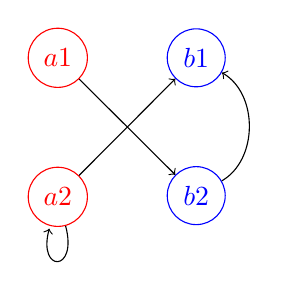
\begin{tikzpicture}
   \node[draw, circle, red] (a1) {$a1$}; 
    \node[draw, circle, red, below = of a1] (a2) {$a2$};
        \node[draw, circle, blue, right = of a1] (b1) {$b1$}; 
    \node[draw, circle, blue, below = of b1] (b2) {$b2$}; 

    \path (a1) edge[->] (b2);
    \path (a2) edge[->] (b1);
    \path (b2) edge[->, bend right =60 ] (b1);
    \path (a2) edge[loop below] ();


\end{tikzpicture}

\end{document}
